\documentclass[0-thesis.tex]{subfiles}

\begin{document}
With the required background information, an architecture for an update mechanism can be
proposed. Four key areas that the architecture must deal with have been identified:

\begin{itemize}
    \item Key distribution and management
    \item Authorization and access control
    \item Means of communication
    \item Upgrading images
\end{itemize}

The architecture must propose solutions for these four areas while complying with SUIT as
much as possible in order to make the architecture interoperable and suitable as a
standard. Certain elements, such as how to locally flip an image and which kinds of
authorization tokens to issue, are implementation dependant. The architecture must however
support different means of achieving these goals and not restrict engineers to one certain
implementation.

Alongside these four key areas is the concern of a devices life cycle from an update
perspective. The life cycle should be intertwined with the mechanisms of the architecture
and show how devices can enroll, communicate, and receive updates throughout their long
expected lifetimes. 

Section~\ref{sec:roles} defines what a server and operator means in the context of the
update mechanism. Section~\ref{sec:key-management} discusses what is needed for devices to
enroll in a PKI and how keys are handled during updates. Section~\ref{sec:authorization}
describes the purpose of issuing authorization tokens, how devices can use them, and who
is to be authorized. Section~\ref{sec:communication} describes how devices, servers, and
operators can communicate and shows an example workflow of communicating an update.
Section~\ref{sec:updates} discusses different means of handling the payload when applying
an update. Section~\ref{sec:device-lifecycle} introduces the notion of a life cycle for
devices, and Section~\ref{ssec:different-architectures} shows different examples of
possible architectures.

\section{Roles}
\label{sec:roles}
This Section~explains the notion of servers and operators in the architecture and their
responsibilities. Section~\ref{ssec:who-is-a-server} covers the topic of servers while
Section~\ref{ssec:who-is-an-operator} covers operators.

\subsection{Who Is a Server and What Do They Do?}
\label{ssec:who-is-a-server}
% Server: dedicated server or other device in network. Identified by keys, needs to be on
% devices? Single point of truth for device profiles and versions. Can be used as storage
% for images being deployed later on.
Servers are responsible for transporting manifests and images to the devices and keeping
track of device profiles. Upon enrollment devices register at a server and the server
creates a profile for that device. The profile contains the vendor and class IDs and
firmware version of the device. This allows the server to know through which protocols the
device can be contacted and which version it should be updated to. Operators, discussed in
the next section, send signed manifests and images to servers, and can query them for
device status.

Devices should contain a list of servers and by trusting the certificate authority, they
can validate those machines certificates after being enrolled. A server is thus any
machine that is enrolled, has a valid certificate, and is included in the devices list of
servers. The reasoning behind this decision is that a standard solution for updates should
not assume the topology of an IoT network. The server may be a machine acting as a proxy
between a traditional network containing the operator and a constrained network with IoT
devices. The server could be a more capable IoT device located entirely within the
constrained network and be contacted through a proxy. The server could be located entirely
within the traditional network and use a proxy to communicate with devices of the
constrained network.

% TODO: Does a device need one keypair for each server? Does it need one keypair for all servers?
A device could also be aware of several servers, and different devices can be mapped to
different servers. This can make device management easier as certain classes of devices
can be handled by certain servers. By allowing a device to receive updates from several
servers, the update mechanism architecture displays a form of robustness. If one server is
a machine located entirely within the constrained network and the connection between that
server and the operator is severed, updates can still be distributed through other
servers. If devices are pulling updates, they can query the servers in order of their list
of servers. If updates are pushed, devices keep the connection with the server pushing the
update.

Which machines are allowed to act like servers can be boiled down to a few important
points no matter the topology of choice:

\begin{itemize}
    \item The server is enrolled and has a valid certificate
    \item The server is included in a devices list of servers (meaning it is authorized to
            transport updates to the device)
    \item An operator can reach the server and is authorized by the server to upload
            updates
\end{itemize}

What servers are allowed to do must also be predetermined. Imagine a device running an
operating system and an application. The operating system is developed by some party
different than the one developing the application, and thus the device is aware of two
update servers, one for the operating system and one for the application. If receiving an
update from the application update server, the device should allow for the update to
happen but also make sure the correct parts of code are updated. The application vendor
should not be allowed to touch the operating system if they are not authorized to do so,
and vice versa. This introduces the topic of authorizing updates. Authorization and access
control is discussed in Section~\ref{sec:authorization}.

\subsection{Who Is an Operator and What Do They Do?}
\label{ssec:who-is-an-operator}
% Operator: human making decisions about updates. Crafts/generates manifests, signs
% manifests and images. Authorized by keys, needs to be on device? Can send manifest for
% ease of operations, cannot send images because of size constraints/single point of
% truth/proxying? How does an operator send manifests, get profile from server? Must get
% profiles anyways for versioning.
Operators are people authorized to upload manifests and images to a server. They can also
optionally upload manifests directly to a device depending on the architecture. Operators
prepare manifests and images and signs them before transporting them to a server, which
forwards them to a device. The signing ensures end-to-end security for images and
manifests between operators and devices.

Like a list of servers introduced in Section~\ref{ssec:who-is-a-server}, devices also need
a list of operators. This is because if an operator wishes to send a manifest directly to
a device, the device needs to know if the operator is authorized to do so, otherwise it is
discarded. Just like with mapping devices to servers, devices can receive manifests from
several operators and different devices may interact with different operators. This
creates opportunities to logically divide a network between different operators. An
example use case is a constrained network supported by different vendors; the respective
vendors should only be able to service their respective devices despite all devices
belonging to the same network. It can also create a hierarchy, where certain operators may
directly interact with devices but other operators must interact with devices through
servers. Yet again the point is to prepare for as many different scenarios as possible and
create a flexible architecture.

As with servers, the essence of being an operator can be captured in a few points:

\begin{itemize}
    \item An operator is enrolled and has a valid certificate
    \item An operator is included in a devices list of operators (and therefore can send
            manifests to the device)
    \item An operator is trusted by a server to send manifests and images to the server,
            causing devices to update
\end{itemize}

Access control for operators is an important topic. Operators should only be able to send
updates to devices they are authorized for, and the updates should cover parts of the
device within the operators rights. Section~\ref{sec:authorization} discusses access
control for operators and servers.

\section{Key Management}
\label{sec:key-management}
% TODO: Mention what is needed for enrollment 
% Consider updates breaking certificates. Why would they? Lack of understanding concerning
% certificates perhaps
% Two pairs of keys from one PSK? Are two pairs needed?
The architecture will, in order to align with the goals of SUIT, be based on asymmetric
cryptography. The availability of EST-coaps makes this feasible in IoT contexts but other
enrollment protocols could also be used. This means a \gls{ca} is needed to act as a
trusted third party distributing certificates. The certificates are linked to a public key
which has a private key partner and are used to verify the correctness of a public key.
Certificates are signed by the CA and in order to trust them, device have to trust the CA
itself.

In order to enroll, a pre-shared key is proposed. This is the approach used in EST-coaps,
but it is not chosen for that reason. If a pre-shared key is not used the CA cannot be
sure the device asking to enroll really should be part of the trusted network. An attacker
that obtained a valid certificate could communicate with devices and servers alike and no
one would be able to tell it is a malicious actor. CAs must know they are issuing
certificates to the correct devices and pre-shared gives devices a means of identifying
themselves. Pre-shared keys could be used for encrypting all traffic but as they are less
scalable and harder to manage than certificates, they are just used for enrolling.

A device that is enrolling has to trust the CA issuing the certificate. If it cannot do
so, how could it know it received a valid certificate? An attacker would love for a device
to use the attackers public key instead, and if an attacker poses as a CA it could issue a
certificate with its own public key and then sign it. In order to trust the CA, a device
needs to have the certificate of the CA it is enrolling with or some other CA further down
the chain of trust. By verifying the signature on the newly enrolled certificate with the
CAs own certificate, a device can be certain they are using the correct keys.

When applying updates, certificates might not be valid anymore. This is implementation
dependant and might not always be a problem, but the architecture should be prepared for
these situations. In the case an update breaks a certificate, the certificate cannot be
used for communication and thus the device cannot use it to re-enroll either. In this
case, a new pre-shared key should be part of the update so that the device can enroll as
if it was factory new. The process of issuing pre-shared keys might be difficult to
automate as the CA must be aware of which keys to accept, but it is needed to ensure the
security of future device communication.

\section{Authorization}
\label{sec:authorization}
A flexible architecture introduces different configurations of server, operators, and
devices. An operator might be authorized to update all parts of all devices, or be
constrained to updating a specific piece of functionality for a subset of the devices.
Servers may only be allowed to update devices manufactured by a specific vendor, and so
on. Controlling access rights is a security issue and the architecture must support it.

% TODO: Image showing how a server authorizes itself using ACE? Mention it assumes already
% enrolled and registered devices. Adapt the RFC image

% TODO: Explain how an authorization server can be used and how it can be placed in or
% between networks. Introspection

% TODO: Discuss if operators, or servers, or both must receive authorization tokens. Argue
% for that only operators do since 1) they are the ones making a decision and 2) updates
% are always at some point prepared by an operator and thus authorized. Servers just act
% as forwarding proxies, image repositories, and profile databases.

\section{Communication}
\label{sec:communication}

% TODO: Update image with:
% Authorization server
% Operator obtaining a token
% Device optionally introspecting it
% Operator preparing manifest
% Maybe break up into two figures if too messy
\begin{figure}
    \caption{Example workflow of communication in the architecture.}
    \label{fig:communication-workflow}
    \begin{tikzpicture}[box/.style={rectangle,draw,minimum width=3cm, minimum height=3.2cm},
        line/.style={->,>=latex}]
        \node[box] (operator) {Operator};
        \node[box, right=3cm of operator] (server) {Server};
        \node[box, right=3cm of server] (device) {Device};
        \node[box, below=1.5cm of server] (CA) {CA};

        \draw[line] (device.south) -- node[above,sloped] {0.0 Enroll} (CA.east); 
        \draw[line] ([yshift=1.5cm]device.west) -- node[above] {0.1 Register} ([yshift=1.5cm]server.east);
        \draw[line] ([yshift=0.8cm]operator.east) -- node[above] {0.3 Manifest}node[below] {Image} ([yshift=0.8cm]server.west);
        
        \draw[line] ([yshift=0.8cm]server.east) -- node[above] {0.4 Manifest and image} ([yshift=0.8cm]device.west);
        \draw[line] ([yshift=-0.8cm]device.west) -- node[above] {0.5, 1.6 Update profile} ([yshift=-0.8cm]server.east);
        
        \draw[line, bend right] (operator.north) to[out=30,in=150] node[above] {1.3 Manifest} (device.north);
        \draw[line] ([yshift=-0.8cm]operator.east) -- node[above] {1.4 Image} ([yshift=-0.8cm]server.west);
        \draw[line] ([yshift=-1.5cm]server.east) -- node[above] {1.5 Image} ([yshift=-1.5cm]device.west);
    \end{tikzpicture}
\end{figure}

Figure~\ref{fig:communication-workflow} shows the proposed architecture and the flow of an update
mechanism. The update mechanism follows the device life cycle and presents two modes of
distributing manifests and images. The steps are numbered 0.0 to 0.6 and 1.7, with the
first three steps being mutual. The modes diverge with step 0.4 and 1.4 respectively. The
common steps for updating a device is as follows:

\begin{enumerate}[label=0.\arabic*]
    \setcounter{enumi}{-1}
    \item Enrolling the device at the certificate authority. This is one half of the
            enrollment stage in the life cycle.
    \item Registering at the server. This is the second half of the enrollment stage
            in the life cycle and creates a profile for the device on the server.
    \item The operator prepares a manifest and signs it.
    \item The operator requests an access token from the authorization server in order to
            gain access to applying updates.
\end{enumerate}

At this point the two modes diverge in how they proceed. Distributing the manifest and
image together works as follows:

\begin{enumerate}[label=0.\arabic*]
    \setcounter{enumi}{2}
    \item The manifest and image are both signed and sent to the server with the
            authorization token. If the image is small enough it can be attached as a
            payload in the manifest itself.
    \item The signed manifest and image are sent with the authorization token to the
            device. If sent in different packets, the manifest can be sent first and the
            image after the device confirms the manifest is correct. The device can either
            query the server for an update, or the server can push the update to the
            device.
    \item The device optionally requests introspection data from the authorization server
            to verify the authorization token.
    \item The device confirms the update if successful and causes the server to update
            its device profile.
\end{enumerate}

If the manifest and image are distributed separately the following steps occur instead of
steps 0.3-0.5:

\begin{enumerate}[label=1.\arabic*]
    \setcounter{enumi}{2}
    \item The signed manifest is sent with the authorization token directly from the
            operator to the device.
    \item The authorization token and signed image is sent to the server.
    \item The authorization token and signed image is sent to the device. This can be done
            either by the device querying the server following a successful manifest parsing,
            or by the server pushing the image to the device.
    \item The device optionally requests introspection data from the authorization server
            to verify the authorization token.
    \item The device confirms the update if successful and causes the server to update
            its device profile.
\end{enumerate}

There are also possibilities regarding how the updating process is initiated. Either the
device could query the server for an update, which prompts a notification to an operator.
Upon notification, an operator can prepare a manifest and image and send to the server as
described above. It is also possible for an operator to query the server for the status of
one or several devices, prepare an update for them, and have the update pushed through the
server. Both approaches assume the devices are already enrolled and registered at the
server.

Whether the manifest and image are distributed together or separately, they are both
signed by the operator in order to achieve end-to-end security between the operator and
device. The server should not be able to decrypt the payloads of manifest and image as
that could enable for instance MITM attacks. The device is to only accept manifests from
either the operator or server, and images from the server. This raises two important
questions: who can act as an operator, and who can act as a server?

\section{Updates}
\label{sec:updates}
% TODO: How to handle decryption and validation
% I like the idea of decrypting once and storing decrypted image with its hash for smaller
% bootloader procedure. Implementation specific though
% Cite mailing list perhaps?


\section{Device Life Cycle}
\label{sec:device-lifecycle}
A network of IoT devices can consist of many different kinds of devices. They may contain
different components, perform different tasks, and thus have different means of
communication. This will impact how they enroll in a secure network and how they
communicate with a server, the server will need to know what protocols and security
measure a specific device handles. It is helpful to think about the life cycle of devices:
how they enroll in a secure network, how they securely communicate with a server, and how
they can be maintained for all those years they are intended to work.

The life cycle of a device can be summarized as in Figure~\ref{fig:lifecycle}. The figure
shows the different stages of a device from being manufactured to ending its service.
There are also annotations showing what needs to be done in each stage. These stages are
discussed in further detail in this section.

\begin{figure}
    \caption{The life cycle of a device.}
    \label{fig:lifecycle}
    \begin{tikzpicture}[>=stealth',
        box/.style={rectangle,draw,minimum width=3cm,minimum height=2cm}]
        \node[box] (new) {Factory new};
        \node[box, below right=1.5cm of new] (enroll) {Enrollment stage};
        \node[box, below left=1.5cm of enroll] (maintain) {Maintenance};
        \node[box, below left=1.5cm of new] (end) {End of life};

        \node[align=left, above right=0.6cm of new] (new_notes) {Ship with:\\
            Pre-shared key\\
            Vendor and class IDs\\
            Server registration endpoint\\
            CA certificate};
        \node[align=left, xshift=-2.5cm, yshift=-1cm, below right=0.4cm of enroll] (enroll_notes) 
            {Register at server/update profile\\
            Obtain certificate};
        \node[align=left, below left=0.7cm of maintain] (maintain_notes) {Push/pull updates};

        \path[->,>=stealth]
        (new) edge [bend left=35] (enroll)
        (enroll) edge [bend left=35] (maintain)
        (maintain) edge [bend left=45] (enroll)
        (maintain) edge [bend left=35] (end);
        
        \def\myshift#1{\raisebox{-2.5ex}}
        \path[decoration={text along path,text align=center,
        text={|\myshift|Please recycle}, raise=0.7cm}]
        (end) edge[decorate, bend left=35] node {} (new);

        \path[->,>=stealth,dashed]
        (end) edge [bend left=35] (new);

        \path[-,>=stealth]
        (new) edge (new_notes)
        (enroll) edge (enroll_notes)
        (maintain) edge (maintain_notes);
    \end{tikzpicture}
\end{figure}

The current state of the SUIT architecture assumes asymmetric cryptography using a PKI,
and with the availability of EST-coaps this is feasible for IoT contexts. The thesis will
therefore propose an architecture based on asymmetric cryptography, but as the SUIT
standard might be further developed to include symmetric cryptography as well, the
architecture should be flexible enough to allow for it.

A factory new device that is to be installed in an IoT network needs some information in
order to enroll and register at a server. As a basis for secure communication, a
pre-shared key and \gls{ca} certificate is needed. The pre-shared key will be used during
enrollment to obtain a key pair, and the certificate is to know the devices own
certificate is issued by the correct CA. Furthermore, a device needs appropriate vendor
and class IDs in order to verify the suitability of updates and to register at servers. In
order to communicate with servers and operators, a device also needs predetermined lists
of servers and operators. 

With a pre-shared key, devices can enter the enrollment stage of the life cycle and
securely enroll and obtain a certificate. In order to trust this certificate, they also
need to be shipped with at least one certificate of the certificate authority, or of some
authority further down the chain of trust. If a device is not equipped with a certificate
it cannot trust the authority when enrolling and thus not be sure it has obtained a valid
certificate or not.

After a device has enrolled, it needs to register at a server. This is because IoT
networks can be heterogeneous, containing different kinds of devices communicating in
different ways. In order for a server to know how to reach a device, the device must tell
the server of its capabilities. As discussed in Section~\ref{ssec:information-model}, the
manifest should contain a vendor and class ID so a device can check if an update is
applicable, this means a device must be aware of its own vendor and class ID for
comparison. These pieces of information can be used to register at a server. Devices must
come prepared with their respective IDs and an endpoint or some other service where they
can register. By for instance POSTing their IDs and current firmware version to a specific
server endpoint, a server can create a profile based on the class of the device, enabling
server initiated communication in the future (pushing updates).

There are alternatives to using device profiles. One alternative is not to keep profiles
on the server, but instead keep a list of known protocols implemented by devices in the
network, and when communicating with a device trying each protocol in sequence. This has
the benefit of not needing to keep a and continuously update profiles, but also has some
issues. One issue is that you still need to keep some state of the devices on the server
regarding firmware version. If the server does not know what the status of device versions
are, it cannot help a human operator decide about deploying updates. 

Another drawback is that devices might implement common protocols but have different
preferences. If two devices implement some common protocols but one of them supports
hardware operations for encrypting one of the protocols, it will prefer using that
protocol with the server, whereas the other device might not. The server will however,
with no information about device preference, try the same sequence of protocols with both
devices. Furthermore, as communication can be unreliable over these networks, the server
cannot know for sure if a device does not respond due to not understanding the protocol
and therefore dropping the packets, or if the response just got lost in transmission. It
is more robust to keep track of which protocols devices support and conform to the
preferences of the constrained devices.

Lastly, instead of using profiles all communication could be initiated from the device
side, meaning updates are only done through a pulling mechanism. This would not enable the
use case of pushing updates which could be critical if a vulnerability must be patched
right away. Operators must be given the choice to push updates to their devices, and thus
servers must be able to initiate contact with devices.

After enrollment and registration has been done, the device enters the maintenance stage.
It can be expected to last for several years in this stage, and this is where the device
receives and applies updates. As updates can change the capabilities of devices, by for
instance implementing a new transport protocol in software, devices should confirm
successful updates at the server so the server can build a new profile for that device. If
an old, inefficient protocol has been replaced by a more efficient version the server
should switch to using the new protocol with the updated device. Furthermore, the server
will act as a source of truth regarding the firmware and software versions running on the
devices. If a device successfully changes version, the server must be aware so that future
updates to that device is of the correct version. This also requires updating of a devices
profile as the device remains in use. 

When updating a device, certificates might have to be re-issued. In the best case, the old
certificate of the device can be used to re-enroll in the PKI. Optionally, operators can
prepare an update with a pre-shared key as if the device was factory new, and let the
device re-enroll. This depends on implementation specific issues such as how keys are
stored in the device and if the device has a file system or not, but it is important to
note that updates might break certificates and after applying an update a device must be
able to re-enroll at the CA.

The device will remain in the maintenance stage until it either breaks or is taken out of
service. If you are a manufacturer of IoT devices please consider recycling or (securely)
re-using devices, starting the life cycle anew.


\section{Different Architectures}
\label{ssec:different-architectures}
As discussed, operators, servers, and devices can interact in many ways. The architecture
tries to be flexible allowing for different network topologies and configurations. The
important parts are that devices can enroll, all actors have valid certificates, and that
devices know which certificates belong to which roles beforehand. 

Figure~\ref{fig:operator-direct} shows an example architecture with one operator, one
server, and one device. The operator is capable of running the protocols needed to
communicate in the constrained network, and can thus interact both directly with the
device to send manifests and interact with the server residing within the constrained
network. A architecture like this allows for servers to be distributed within the
constrained network.

\begin{figure}
    \caption{An operator communicating directly with machines in the constrained network.}
    \label{fig:operator-direct}
    % TODO: Placeholder image
    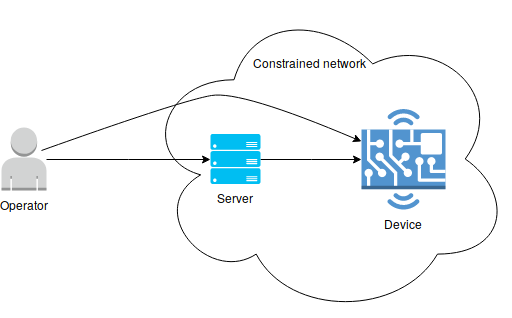
\includegraphics[scale=0.8]{images/operator-direct.png}
\end{figure}

Figure~\ref{fig:operator-proxy} shows an operator interacting with a proxy which in turn
interacts with the server. Note that since the operator is not capable of contacting the
server directly it can not contact the device directly either. All traffic, manifest and
image, goes through the server to the device. 

\begin{figure}
    \caption{An operator using a proxy to reach the constrained network.}
    \label{fig:operator-proxy}
    % TODO: Placeholder image
    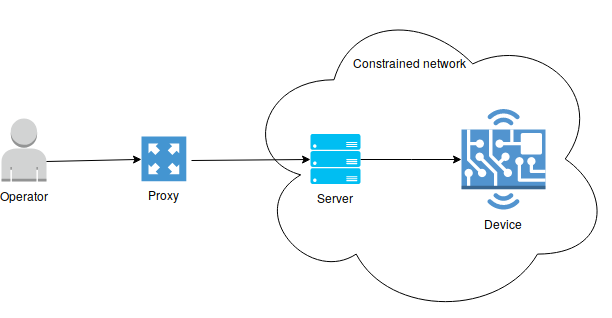
\includegraphics[scale=0.7]{images/operator-proxy.png}
\end{figure}

Figure~\ref{fig:operator-server} shows a third alternative where the server acts as a
proxy between the operator and the device. The operator is yet again unable to reach the
devices directly and relies on a server. In this scenario, there are two devices who both
receive updates from the server. If the devices use the same transport protocols,
broadcasting could be used from the server to send updates to both devices at the same
time.

\begin{figure}
    \caption{A server is used as a proxy to reach two devices.}
    \label{fig:operator-server}
    % TODO: Placeholder image
    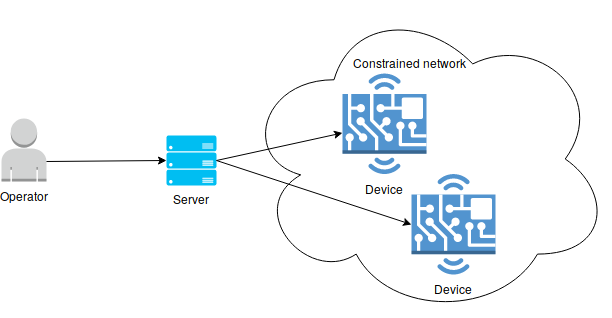
\includegraphics[scale=0.8]{images/operator-server.png}
\end{figure}

There are many other possible architectures and configurations. What these three examples
have in common is that the operator always resides outside the constrained network,
devices always reside within the constrained network, and that servers transport images to
devices. In turn, devices register and update their statuses to the servers. Since
operators reside in traditional networks using traditional protocols such as HTTP over
TCP, a proxy mechanism may be necessary to communicate with the often UDP based
constrained networks. Remember from Section~\ref{ssec:coap} that CoAP can easily be
proxied to and from HTTP meaning a server running for instance CoAP could also be used as
a proxy for the operator. If the operator has the proper protocols implemented, they could
communicate manifests directly to a device.

\end{document}